\documentclass[12pt,oneside]{book}

% PACCHETTI
\usepackage{hyperref}           % hyperlinks
\usepackage{tabto}              % strumento per inserire tab nel testo
\usepackage[                    % geometria della pagina
    a4paper,
    inner=2cm,
    outer=3cm,
    top=3cm,
    bottom=3cm,
    bindingoffset=1.2cm
]{geometry}
\usepackage[utf8]{inputenc}     % 3 pacchetti per l'italiano
\usepackage[italian]{babel}
\usepackage[T1]{fontenc}
\usepackage{titlesec}           % custom chapter titles

\usepackage{fancyhdr}
\usepackage{multicol}
\usepackage[arrowdel]{physics} 
\usepackage{amsmath}

\usepackage{graphicx}           % IMMAGINI
\graphicspath{ {./images/} }


% INFORMAZIONI SUL DOCUMENTO
\title{\Large{\textbf{Fisica 1}}}
\author{Enrico Bragastini}
\titleformat{\chapter}[display]{\normalfont\bfseries}{}{0pt}{\LARGE}


% CONTENUTO
\begin{document}
\pagestyle{fancy}
\fancyhf{}
\rhead{}
\lhead{\nouppercase\leftmark}
\cfoot{\thepage}
\frontmatter

% Prima pagina - Titolo
\maketitle
\tableofcontents

\mainmatter
\chapter{Nozioni di base}
\section{Misura di una grandezza}
Una \textbf{grandezza fisica} è la proprietà di un fenomeno, corpo o sostanza, che può essere espressa
quantitativamente mediante un numero e un riferimento.

\noindent La misura di una grandezza può avvenire con due modalità:
\begin{itemize}
    \item Mediante un dispositivo sperimentale
    \item Confronto con un'altra grandezza omogenea di riferimento e costante
\end{itemize}

\noindent L'espressione di una grandezza fisica avviene nella forma:
\begin{equation*}
    \text{Numero} + \text{\underline{\emph{Unità di misura}}}
\end{equation*}

\section{Grandezze fisiche fondamentali e derivate}
Possiamo distinguere le grandezze fisiche in \underline{fondamentali} e \underline{derivate}.

\noindent Le \textbf{grandezze fisiche fondamentali} sono:
\begin{itemize}
    \item Lunghezza                 \tabto{7cm} [L]
    \item Massa                     \tabto{7cm}  [M]
    \item Tempo                     \tabto{7cm}  [t]
    \item Intensità Di Corrente     \tabto{7cm}  [i]
    \item Temperatura Assoluta      \tabto{7cm}  [T]
\end{itemize}

\noindent Le \textbf{grandezze fisiche derivate} sono grandezze che possono essere
espresse in forma di combinazioni matematiche delle grandezze fondamentali.
Alcuni esempi di grandezze derivate sono:
\begin{itemize}
    \begin{multicols}{2}
        \item Superficie
        \item Volume
        \item Velocità
        \item Accelerazione
        \item Forza
        \item Pressione
    \end{multicols}
\end{itemize}

\section{Sistemi di Unità di Misura}
\begin{center}
    \bgroup
    \def\arraystretch{1.5}
    \begin{tabular}{ |c| c c c c c|}
        \hline
        SISTEMA     & Lunghezza & Massa & Tempo & Corrente & Temperatura \\
        \hline
        MKS (s. i.) & m         & kg    & s     & A        & °K          \\
        \hline
        cgs         & cm        & g     & s     & A        & °K          \\
        \hline
    \end{tabular}
    \egroup
\end{center}

\subsection{Ulteriori Unità di Misura}
Esistono ulteriori sistemi di unità di misura che permettono di avere maggiore comodità
nelle misurazioni di particolari grandezze.
Se ne elencano alcuni:

\begin{enumerate}
    \item Lunghezza:    \tabto{3cm} Ångströms, Anno-Luce
    \item Tempo:        \tabto{3cm} Minuto, Ora
    \item Volume:       \tabto{3cm} Litro
    \item Velocità:     \tabto{3cm} Chilometro/Ora
    \item Pressione:    \tabto{3cm} Atmosfera, Millimetro di mercurio
    \item Energia:      \tabto{3cm} Elettrovolt, Chilovattora
\end{enumerate}

\section{Notazione Scientifica}
Per i numeri particolarmente grandi o piccoli risulta comodo rappresentarli
in \textbf{Notazione Scientifica} utilizzando le potenze del 10.

La notazione scientifica permette di scrivere un numero in cui compare una sequenza molto lunga di zeri in forma compatta.
In matematica si dice che un numero è scritto in notazione scientifica se è della forma $n\cdot10^e$

~\newline
\underline{Esempio:}
\begin{equation*}
    1,2 \cdot 10^5
\end{equation*}
Un numero in \emph{notazione scientifica} è quindi composto da:
\begin{itemize}
    \item Un numero compreso n tale che $1 \leq n < 10$
    \item Una potenza del 10 con esponente intero
\end{itemize}

\newpage
\section{Analisi Dimensionale}
Quando si è di fronte ad una formula fisica o si svolgono calcoli con grandezze fisiche e unità di misura,
per verificare la plausibilità della formula data e la consistenza
dei calcoli svolti si può ricorrere all'analisi dimensionale.

Eseguire l'analisi dimensionale di una formula, o più in generale di un'equazione fisica,
vuol dire ricavare le dimensioni di ognuno dei due membri allo scopo di verificare che esse coincidano:
se così non fosse ci sarebbe necessariamente qualcosa di sbagliato, perché avremmo a che fare con un'equazione
dimensionalmente non consistente.


\section{Sistemi di Coordinate}
Molti aspetti della fisica hanno in qualche modo a che fare con la descrizione di un punto dello spazio.
Ad esempio, la descrizione matematica del moto di un corpo richiede un metodo che descriva la successione
delle posizioni occupate dal corpo nel tempo.

\subsection{Coordinate cartesiane}
In due dimensioni questa descrizione può essere realizzata con l’uso di un sistema di \textbf{coordinate cartesiane}
in cui due assi perpendicolari si intersecano in un punto definito come punto origine.
Le coordinate cartesiane sono anche dette \emph{coordinate rettangolari}.
\begin{figure}[h]
    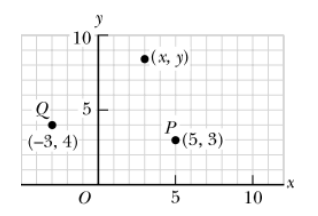
\includegraphics[scale=0.5]{coordinate_cartesiane}
    \centering
\end{figure}

\subsection{Coordinate scalari}
Talvolta è più conveniente rappresentare un punto in un piano tramite le sue \textbf{coordinate polari piane} $(r, \theta)$.

\begin{figure}[h]
    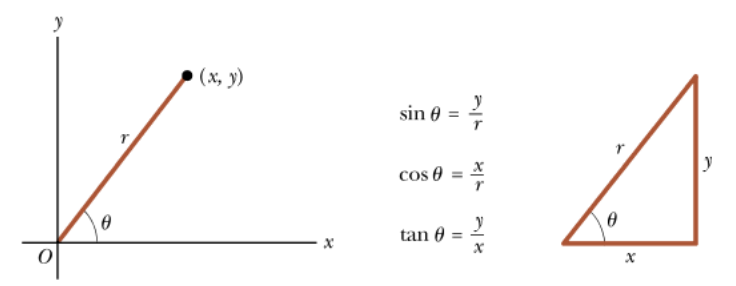
\includegraphics[scale=0.5]{coordinate_polari}
    \centering
\end{figure}
In questo sistema di coordinate polari, r è la distanza dall’origine al punto di coordinate
cartesiane $(x, y)$ e $\theta$ è l’angolo fra un asse fisso e la semiretta tracciata dall’origine al punto, generalmente
misurato in verso antiorario dall’asse x positivo.

\paragraph{Conversione delle coordinate} Partendo dalle coordinate polari, si possono ottenere le coordinate cartesiane
tramite le seguenti equazioni:
\begin{itemize}
    \item $x = r \cdot \cos{\theta}$
    \item $y = r \cdot \sin{\theta}$
\end{itemize}
Inoltre, sfruttando la trigonometria si possono ottenere queste altre informazioni:
\begin{itemize}
    \item $\tan{\theta} = \frac{y}{x}$
    \item $r = \sqrt{x^2 + y^2}$
\end{itemize}

\section{Grandezze scalari e grandezze vettoriali}

\subsection{Grandezza scalare}
Una \emph{grandezza scalare} è una grandezza che è specificata solamente da un valore con una certa unità di misura e non associata con una direzione.

Alcune grandezze scalari sono \emph{sempre positive}, come la massa e la velocità scalare.
Altre, come la temperatura, possono avere valori \emph{sia positivi che negativi}.
Per manipolare le quantità scalari si adoperano le \textbf{normali regole dell’aritmetica}.

\subsection{Grandezza vettoriale}
Una grandezza vettoriale è una grandezza che, per essere specificata,
ha bisogno sia di un numero con le sue unità di misura (\textbf{modulo del vettore}), sia di una \textbf{direzione orientata}.

Per rappresentare un vettore, si utilizza una lettera sormontata da una freccia come da esempio:
\begin{equation*}
    \vec{A}
\end{equation*}

\newpage
\section{Proprietà e operazioni con i vettori}
\subsection{Uguaglianza di due vettori}
Due vettori $\vec{A}$ e $\vec{B}$ sono \textbf{uguali} se sono uguali i loro \emph{moduli}, la \emph{direzione} e il \emph{verso}.
L'uguaglianza è \emph{indipendente dall'origine}, ovvero i vettori possono essere traslati sul grafico in base alla necessità
senza che venga persa la loro uguaglianza.
\begin{figure}[h]
    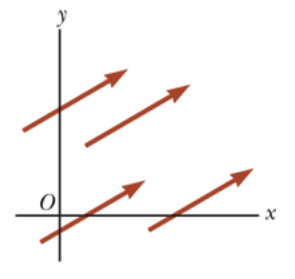
\includegraphics[scale=0.5]{uguaglianza_vettori}
    \centering
\end{figure}

\subsection{Somma tra vettori (metodo grafico)}
La somma tra vettori può essere svolta rapidamente in modo grafico.

In generale, se si vogliono sommare due spostamenti rappresentati dai due vettori $\vec{a}$ e $\vec{b}$ come di seguito rappresentato:
\begin{figure}[h]
    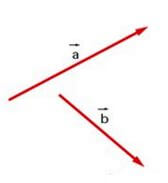
\includegraphics[scale=0.5]{vettori_da_sommare}
    \centering
\end{figure}

\paragraph{Metodo punta-coda:} Spostiamo uno dei due vettori in modo tale che la sua coda coincida con la punta del primo vettore.

~\newline
\noindent Riferendoci al nostro caso, spostiamo il vettore $\vec{b}$ vettore in modo tale che la sua coda coincida con la
punta del vettore $\vec{a}$, come di seguito rappresentato:
\begin{figure}[h]
    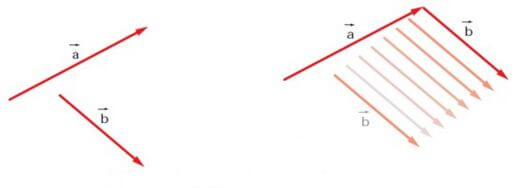
\includegraphics[scale=0.5]{punta_coda}
    \centering
\end{figure}

Come è possibile notare dalla figura precedente lo spostamento del vettore $\vec{b}$ deve essere effettuato in modo
tale che la freccia rimanga sempre parallela a se stessa.
Lo spostamento totale si ottiene unendo la coda del vettore $\vec{a}$ con la punta del vettore $\vec{a}$, come di seguito
rappresentato:
\begin{figure}[h]
    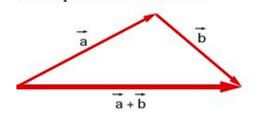
\includegraphics[scale=0.5]{vettori_sommati}
    \centering
\end{figure}

Si noti che in generale il modulo del vettore somma non è uguale alla somma dei moduli dei singoli spostamenti.

\subsection{Opposto di un vettore}
L'\textbf{opposto di un vettore} $\vec{A}$ è definito come il vettore che sommato a $\vec{A}$ permette di ottenere 0.
\begin{equation*}
    \vec{A} + (- \vec{A} ) = 0
\end{equation*}
Il vettore $(-\vec{A})$ è quindi un vettore che ha lo \textbf{stesso modulo} di $\vec{A}$, con la \textbf{stessa direzione} ma di \textbf{verso opposto}.

\subsection{Sottrazione tra vettori}
La \textbf{sottrazione tra vettori} si ottiene sfruttando la definizione di \emph{vettore opposto}.
Quindi, si vuole sottrarre il vettore $\vec{B}$ al vettore $\vec{A}$, basta \emph{sommarne l'opposto}.
\begin{equation*}
    \vec{A} - \vec{B} = \vec{A} + (- \vec{B})
\end{equation*}

\subsection{Prodotto tra un vettore e uno scalare}
\begin{itemize}
    \item Se un vettore $\vec{A}$ viene moltiplicato per una quantità scalare positiva $m$,
          allora il prodotto è $m\vec{A}$ e possiede la stessa direzione di A e modulo $mA$.
    \item Se un vettore $\vec{A}$ viene moltiplicato per una quantità scalare negativa $-m$,
          allora il prodotto è $-m\vec{A}$ e possiede direzione opposta di A e modulo $mA$.
\end{itemize}

\newpage
\section{Componenti di un vettore e vettori unitari}
\subsection{Componenti di un vettore}
Il metodo geometrico di somma vettoriale non è raccomandabile in quelle situazioni in cui si richiede una precisione elevata, oppure nei problemi in tre dimensioni.
Esiste un metodo per sommare i vettori che fa uso delle \emph{proiezioni dei vettori} lungo gli assi coordinati.
Queste proiezioni sono chiamate \textbf{componenti del vettore} o anche componenti rettangolari del vettore. Un vettore può essere descritto in modo completo dai suoi componenti.

Un vettore $\vec{A}$ può essere espresso come come \emph{somma di due vettori componenti}: $\vec{A_x}$, parallelo all'asse $x$, sommato a $\vec{A_y}$,
parallelo all'asse $y$.
\begin{figure}[h]
    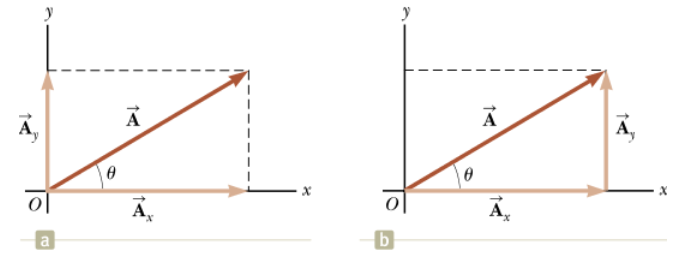
\includegraphics[scale=0.5]{vettori_componenti}
    \centering
\end{figure}

\noindent Si ottengono quindi le seguenti relazioni:
\begin{itemize}
    \item $\vec{A} = \vec{A_x} + \vec{A_y}$
    \item $\vec{A_x} = A \cos{\theta}$
    \item $\vec{A_y} = A \sin{\theta}$
    \item $A = \sqrt{A_x^2 + A_y^2}$
    \item $\theta = \tan[-1](\frac{A_y}{A_x})$
\end{itemize}
Nell’affrontare un problema fisico si può scegliere di specificare un vettore $\vec{A}$
per mezzo delle sue componenti $\vec{A_x}$ e $\vec{A_y}$ oppure per mezzo del suo modulo A e dell’angolo $\theta$.

\subsection{Vettori unitari}
Un \textbf{vettore unitario} è un \emph{vettore adimensionale} il cui modulo è esattamente 1.
I vettori unitari hanno l'unico scopo di indicare una direzione orientata e non hanno nessun altro significato fisico.
Il modulo dei vettori unitari è uguale a 1, ovvero $\abs*{\hat{i}} = \abs*{\hat{j}} = \abs*{\hat{k}} = 1$

Useremo i simboli $\hat{i}$, $\hat{j}$, e $\hat{k}$ per rappresentare i vettori unitari che puntano rispettivamente nelle direzioni positive x, y e z.

\newpage
\begin{figure}[h]
    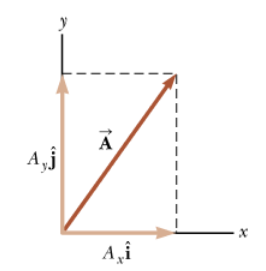
\includegraphics[scale=0.5]{vettori_unitari}
    \centering
\end{figure}
Consideriamo un vettore $\vec{A}$ che giace nel piano $xy$ come in figura. 
Il prodotto della componente $A_x$ per il vettore unitario $\hat{i}$ è il vettore $\vec{A_x} = A_x \hat{i}$ parallelo all'asse delle $x$ e di modulo $\abs{A_x}$. 
Analogamente, $\vec{A_y} = A_y \hat{j}$ è un vettore di modulo $\abs{A_y}$ parallelo all’asse $y$. 
Così, nella notazione dei vettori unitari, il vettore $\vec{A}$ è
\begin{equation*}
    \vec{A} = A_x \hat{i} \cdot A_y \hat{j}
\end{equation*}

\subsection{Somma tra vettori (metodo con vettori unitari)}
Quando il metodo grafico non risulta sufficientemente accurato ci si può avvalere dell'utilizzo delle componenti dei vettori da sommare.

Si supponga di voler sommare il vettore $\vec{A}$ composto da $\vec{A_x}$ e da $\vec{A_y}$ al vettore $\vec{B}$
composto da $\vec{B_x}$ e da $\vec{B_y}$.

\begin{figure}[h]
    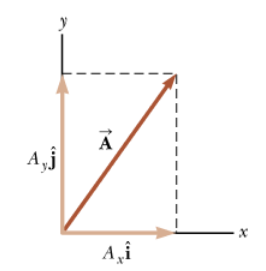
\includegraphics[scale=0.5]{vettori_unitari}
    \centering
\end{figure}

\noindent Per effettuare questa somma basta sommare separatamente le componenti $x$ e $y$. Il vettore risultante $\vec{R} = \vec{A} + \vec{B}$
si ottiene con:
\begin{equation*}
    \vec{R} = (A_x \hat{i} + A_y \hat{j}) + (B_x \hat{i} + B_y \hat{j})
\end{equation*}
ovvero
\begin{equation*}
    \vec{R} = (A_x+ B_x) \hat{i} + (A_y + B_y) \hat{j}
\end{equation*}

~\newline
\noindent Il vettore ottenuto può essere a sua volta visto come $\vec{R} = R_x \hat{i} + R_y \hat{j}$.



\chapter{Cinematica}

La \textbf{Cinematica} è un ramo della \textbf{meccanica classica} che si occupa di descrivere quantitativamente il moto dei corpi, indipendentemente dalle cause del moto stesso.

\section{Moto in una dimensione}

\paragraph{Punto materiale}
Nello studio del moto traslatorio utilizziamo il modello \textbf{punto materiale} e descriviamo il moto di un corpo approssimandolo ad 
“una particella” senza considerare le sue dimensioni reali.

In generale un punto materiale è quel corpo che \emph{ha una massa} ma \emph{ha dimensioni infinitesimali}. 

\section{Posizione, spostamento e distanza}

\paragraph{Posizione} Indichiamo come posizione il punto occupato \emph{istante per istante} dal punto materiale oggetto di studio.
Un corpo è considerato \emph{in moto} se la sua posizione cambia con il passare del tempo.

\paragraph{Spostamento} Lo spostamento, indicato con $\Delta x$\footnote{La lettera greca $\Delta$ indica in generale una \emph{variazione}} è definito come la variazione della sua posizione in un certo intervallo di tempo.

Se da $x_i$ il punto materiale raggiunge la posizione $x_f$ il suo spostamento è definito come la posizione finale meno la posizione iniziale:
\begin{equation*}
    \Delta x = x_f - x_i
\end{equation*}
Lo spostamento è una \emph{grandeza vettoriale}, ma sul moto rettilineo è possibile considerarlo come una \emph{lunghezza scalare}.

\paragraph{Distanza percorsa}
La distanza percorsa \emph{non è lo spostamento}. La distanza indica la lunghezza del cammino percorso da una particella.

Supponiamo che un'automobile parta dal punto $A$, arrivi al punto $B$ e poi ritorni al punto $A$. In questo caso abbiamo che lo spostamento 
è nullo, infatti $x_i = x_f$, ovvero $\Delta x = 0$. Mentre la distanza percorsa corrisponde a $2 (B-A)$.

\section{Velocità media e istantanea}

\paragraph{Velocità media}
La \textbf{velocità media}, $v_{m}$ di un punto materiale, è definita come il rapporto tra lo spostamento $\Delta x$ del punto materiale 
e l’intervallo di tempo $\Delta t$ durante il quale lo spostamento è avvenuto:
\begin{equation*}
    v_{x,media} \equiv \frac{\Delta x}{\Delta t}
\end{equation*}

\begin{itemize}
    \item L'unità di misura è: $\frac{m}{s}$
    \item Se $\Delta x > 0$ (spostamento nel verso positivo), allora $v_m > 0$. 
    \item Se $\Delta x < 0$ (spostamento nel verso negativo), allora $v_m < 0$
\end{itemize}

\paragraph{Velocità media scalare}
La velocità scalare media $v_{media}$ di un punto materiale, una quantità scalare, è definita come il rapporto
fra la distanza totale $d$ percorsa e l’intervallo di tempo impiegato a percorrerla:
\begin{equation*}
    v_{m} \equiv \frac{d}{\Delta t}
\end{equation*}

\paragraph{Velocità istantanea}
La velocità istantanea $v_x$ di un corpo in un determinato istante di tempo $t$ è uguale al valore limite del rapporto $\frac{\Delta x}{\Delta t}$
quando $\Delta t$ tende a $0$. Nel linguaggio del calcolo differenziale questo limite è la derivata di x rispetto a t:
\begin{equation*}
    v_x \equiv \lim_{\Delta t \to 0} \frac{\Delta x}{\Delta t} = \frac{dx}{dt}
\end{equation*}

~\newline
\underline{Esempio:} \newline
Espressione analitica dello spostamento di un punto materiale: $x=-4t + 2t^2$
Calcolo della velocità istantanea a $t = 2,5s$
\begin{align*}
    x &= -4t + 2t^2 \\
    \frac{dx}{dt} &= -4 + 4t \\ 
    v_x &= 6 \; m/s
\end{align*}

\section{Moto Rettilineo Uniforme}
Un corpo si muove con \textbf{moto rettilineo uniforme} quando si sposta lungo una retta con velocità costante.

Basandoci su questa definizione si possono ricavare le seguenti equazioni:
\begin{itemize}
    \item $v_x = \text{costante}$
    \item $v_{x,media} = v_x$
    \item $v_x = \frac{\Delta x}{\Delta t} = \frac{x_f - x_i}{t_f - t_i}$
    \item $x_f = x_i + \frac{v_x(t_f - t_i)}{v_x \Delta t}$, scegliendo \tiny $\begin{aligned} t_i&=0 \\ t_f&=t \end{aligned}$ \normalsize otteniamo $x_f = x_i + v_x \cdot t$
\end{itemize}

\section{Accelerazione media e istantanea}

\paragraph{Accelerazione media} Quando la velocità cambia nel tempo, si dice che la particella sta accelerando.
L’accelerazione media $a_{x,media}$ del punto materiale è definita come la variazione della velocità 
$\Delta v_x$ divisa per l’intervallo di tempo $\Delta t$ in cui avviene la variazione:
\begin{equation*}
    a_{x,media} \equiv \frac{\Delta v_x}{\Delta t} = \frac{v_{xf} - v_{xi}}{t_f - t_i   }
\end{equation*}
L'unità di misura dell'accelerazione è $m/s^2$

\paragraph{Accelerazione instantanea} Si definisce l'accelerazione istantanea come il limite dell'accelerazione
media quando $\Delta t$ tende a zero.
\begin{equation*}
    a_{x,media} \equiv \lim_{\Delta t \to 0} \frac{\Delta v_x}{\Delta t} = \frac{dv_x}{dt} = \frac{d}{dt} (\frac{dx}{dt}) = \frac{d^2x}{dt^2}
\end{equation*}
L’accelerazione istantanea è la derivata della velocità rispetto al tempo che è anche la pendenza della curva del grafico velocità–tempo.

\section{Moto rettilineo uniformemente accelerato}
Nel caso del \textbf{moto rettilineo uniformemente accelerato}, il moto del \emph{punto materiale} avviene con \emph{accelerazione costante}.

Di conseguenza l'accelerazione media e istantanea coincidono.

Basandoci sulla definizione di questo moto si ricavano le seguenti equazioni:
\begin{itemize}
    \item $a_{x,media} = \frac{v_{xf}-v_{xi}}{t_f-t_i} \rightarrow a_x=\frac{v_{xf}-v_{xi}}{t-0}$ 
    \item $v_{x,f} = v_{x,i} + a_{x}t$
\end{itemize}













\end{document}
